

\section{Problem 4}
\label{part4}
\begin{verbatim}
Extra credit, 1 point:

Repeat question #2, but change ``followers'' to ``following''?  In
other words, are the people I am following following more people?

\end{verbatim}

\subsection{Solution}
\begin{enumerate}
\item This question is similar to the second question. There I used ``followers'' and here I need to use ``following''.
\item I choose the source account as my account(``dineshpaladhi'') because I have 186 people following me.
\item So, this should prove that ``people I am following following more people?''
\item To make it more understandable, here I used ``friends'' to represent ``following'' people .
\item Python code is same for this except for the api object we use. Earlier I used api.followers in order get followers and now I used api.friends in order to get the list of people I am following. Python code for this can be seen here \ref{lst:q3-1}.
\item First csv file can be found here \ref{Sample_t3} and it contains the friends screen name and their friends count along with my friends count.
\item Second csv file can be found here \ref{Sample_t4} and it does not contains my friends count.
\item R code for calculating mean,mode and standard deviation can be seen here \ref{lst:q3R}.
\item R code for bar plot can be seen here \ref{2nd:q3R} and my friends count is indicated with a blue arrow mark in the graph so that we can visually see friendship paradox.This can been seen in \ref{graph3}.
\item The Mean I calculated is 8292.253 and the following people count of ``dineshpaladhi'' is 186. Therefore following people count of ``dineshpaladhi'' is less than the Mean which shows that ``dineshpaladhi's'' friends have more friends than ``dineshpaladhi''. 
\item This proves Friendship Paradox using Twitter's following list.
\end{enumerate}
\newpage

\subsection{Code Listing}

\subsubsection{Python Code for getting Twitter friends and their count of friends}
\lstinputlisting[language=Python,breaklines = true,frame=single,caption={Python Code for getting Twitter friends and their count of friends}, label=lst:q3-1,captionpos=b,numbers=left,showspaces=false,showstringspaces=false,basicstyle=\footnotesize]{twit_following.py}
\newpage

\subsection{Results}

\subsubsection{Sample list of Twitter friends and their count with ``dineshpaladhi'' }
\begin{figure}[ht]    
    \begin{center}
        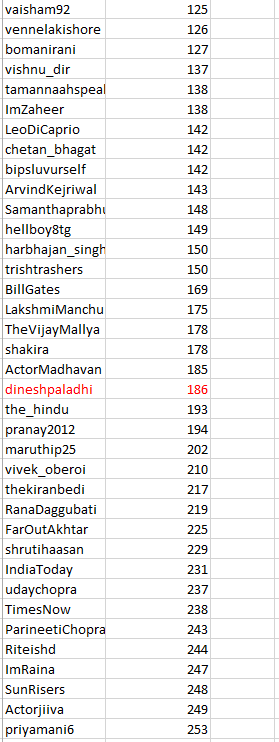
\includegraphics[scale=0.9]{sample_following_with_source.png}
        \caption{Sample list of Twitter friends and their count with source}
        \label{Sample_t3}
    \end{center}
\end{figure}
\newpage
\subsubsection{Sample list of Twitter friends and their count without ``dineshpaladhi''}
\begin{figure}[ht]    
    \begin{center}
        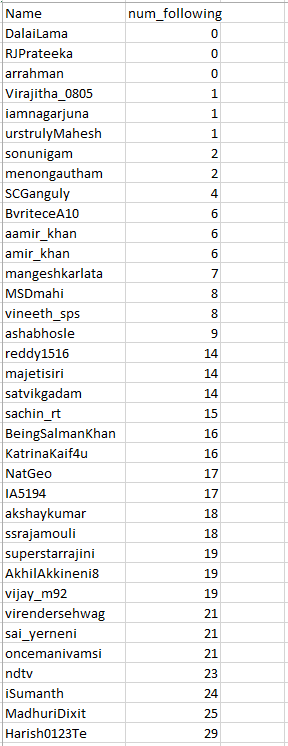
\includegraphics[scale=0.9]{sample_following_without_source.png}
        \caption{Sample list of Twitter friends and their count without source}
        \label{Sample_t4}
    \end{center}
\end{figure}
\newpage
\subsubsection{R code and results for Calculation of Mean,Median and Standard Deviation}
\lstinputlisting[language=R,breaklines = true,frame=single,caption={R code for Mean,Median and Standard Deviation}, label=lst:q3R,captionpos=b,numbers=left,showspaces=false,showstringspaces=false,basicstyle=\footnotesize]{calcul_twit_following.R}

\subsubsection{R code and results for plotting graph between Twitter friends and their count of friends}
\lstinputlisting[language=R,breaklines = true,frame=single,caption={R code for plotting graph between Twitter friends and their count of friends}, label=2nd:q3R,captionpos=b,numbers=left,showspaces=false,showstringspaces=false,basicstyle=\footnotesize]{following_graph_code.R}
\newpage
\subsubsection{Graph showing Twitter friends and their count of friends}
\begin{figure}[ht]    
    \begin{center}
        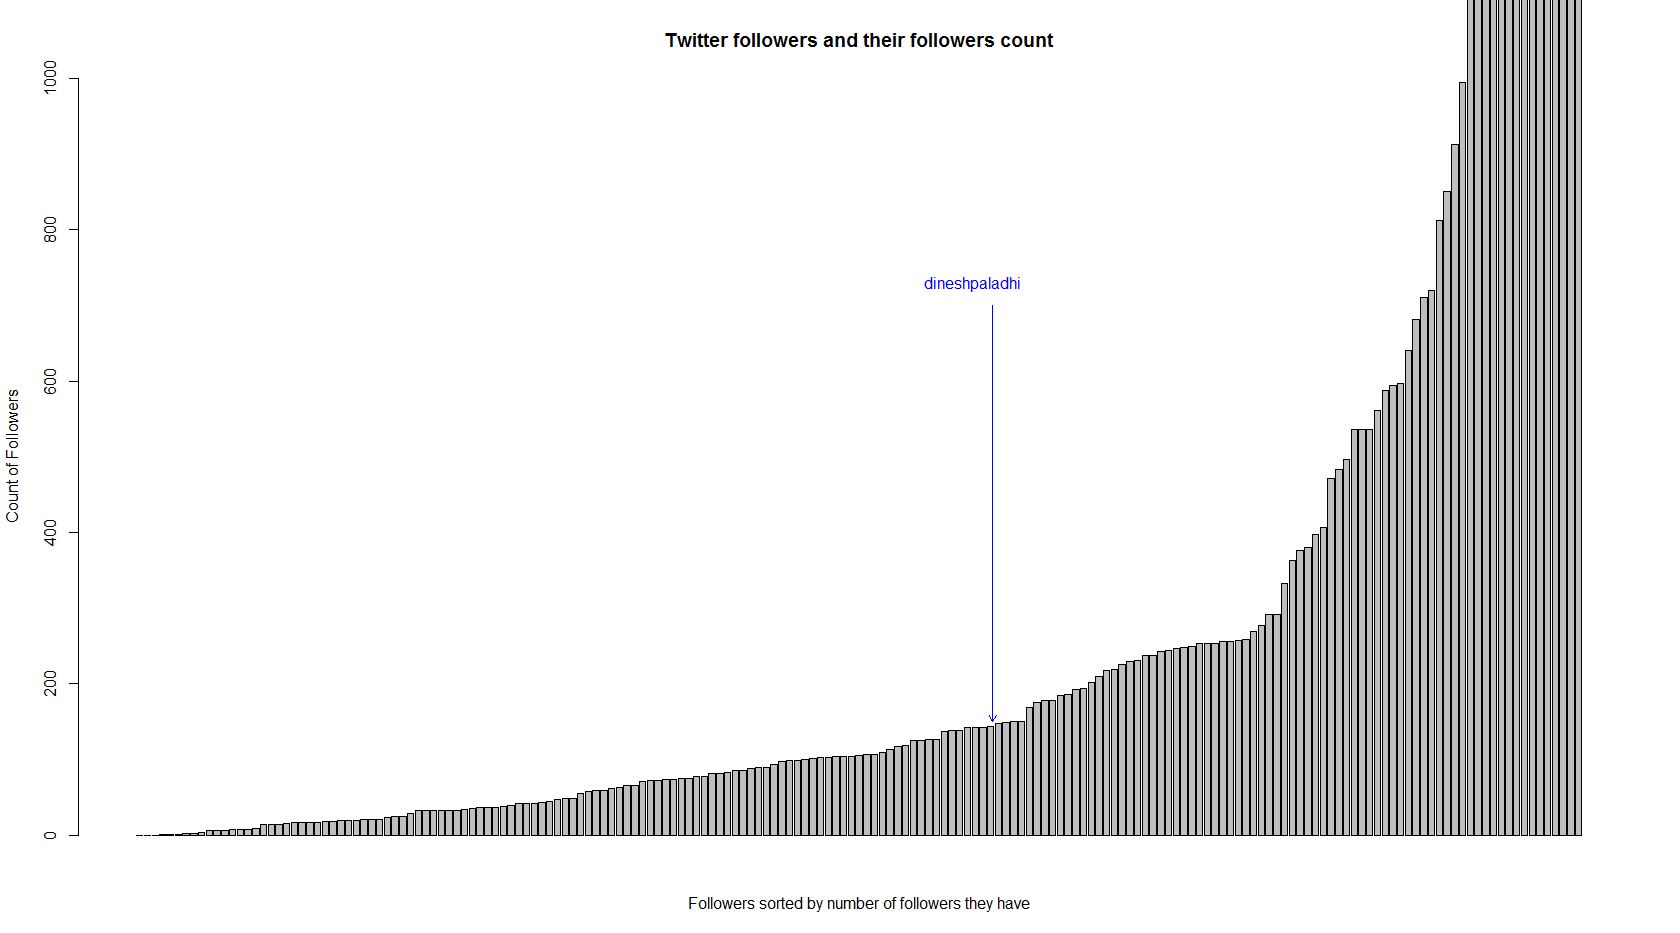
\includegraphics[scale=0.3]{followinggraph.png}
        \caption{Twitter friends and their count of friends}
        \label{graph3}
    \end{center}
\end{figure}
\newpage

